\subsection{miRNA abundance does not predict which miRNAs the CNN ranks well (ENCODE; negative)}
CLIP labels need AGO loaded with the miRNA, so abundant miRNAs could give cleaner labels and higher per-miRNA AUROC. We measured abundance from 21 ENCODE GRCh38 microRNA-seq quantification files covering 12 cell lines (accessions in \texttt{results/encode\_mirna\_abundance.json}; Ensembl REST \texttt{lookup/id} for gene symbols; \texttt{scripts/encode\_mirna\_abundance.py}; hermetic tests). Per file we take $a_g=\log_2(\mathrm{CPM}_g+1)$, sum precursor loci per mature miRNA (precursor counts cannot separate the 5p and 3p arms), average replicates and take the median across lines.
Gates: every file has at least 1{,}500 gene rows; miR-21 sits in the panel's top decile (17.8 vs threshold 12.3); 131/131 panel miRNAs map to a precursor. The pre-registered tissue gate failed: we expected miR-122 to peak in HepG2, but it is zero in all 12 lines. We record that failure and do not retune it. A replacement control chosen after the failure (post-hoc, not pre-registered) passes: MIR142's top three lines are the three blood lines (GM12878, HL-60, K562), and MIR302A, MIR302B and MIR367 each peak in H1 embryonic stem cells.
All three hypotheses are falsified on $n=131$ miRNAs: abundance versus CNN AUROC $\rho=0.076$ ($p=0.195$), versus the CNN's gain over site-count covariates $\rho=0.099$ ($p=0.130$), and the partial correlation given $\log n_{pos}$ $\rho=0.050$ ($p=0.284$; Figure~\ref{fig:encode}). Abundance is also unrelated to the covariate-only AUROC ($\rho=0.010$). A caveat: ENCORI CLIP pools many cell types, and none of the 12 ENCODE lines is HEK293, so a cell-matched abundance could still matter.
\begin{figure}[h]\centering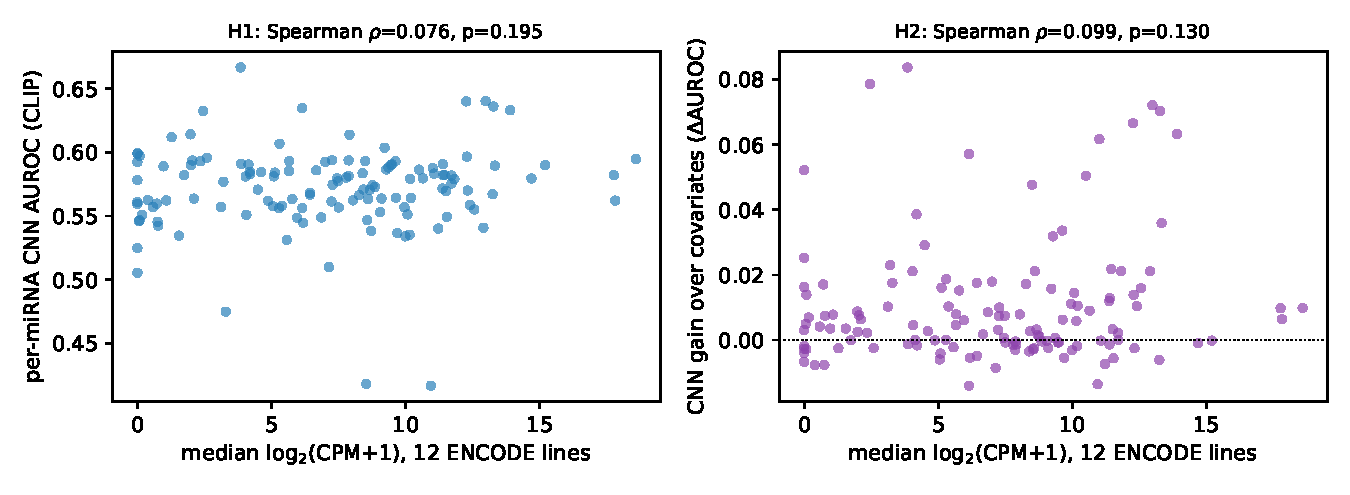
\includegraphics[width=0.95\linewidth]{figs/fig_encode_mirna.pdf}
\caption{Per-miRNA ENCODE abundance (median over 12 cell lines) versus CNN AUROC on CLIP labels (left) and versus the CNN's gain over site-count covariates (right).}\label{fig:encode}\end{figure}
